\chapter{Review of Related Literature}
\section*{On Weak and Easy Notions of Soundness in RDLTs}
Recent formalizations on the definition of weak and easy soundness of RDLT and their structural and behavioral profiles allow the basis for the verification of the said properties. The following definitions are from \cite{Ramirez2024} and contains the weak and easy notions of soundness, its behavioral and structural profiles, and the proposed algorithms for the verification (and the time and space complexity) thereof based on each notion's definitions.
The information under this section is taken from the fundamental work of \cite{Ramirez2024} unless explicitly stated otherwise.
% ---------------------------
% Weak Soundness Notion of RDLTs
\section{Weak Soundness Notion of RDLTs}

\begin{defn}[\textbf{Weak Soundness of RDLTs}] 
    \label{WeakRDLTDef}
    An RDLT $ R $ is of weak soundness if and only if the following requirement is satisfied by each activity profile $ S = \{S(1), S(2), ..., S(k)\}, 1 \leq k \leq diam(R), diam(R) $ is the diameter of $ R $, of a set of source vertices $ I $ $ \subset $ $ V $ and a final output vertex $ f $ $ \in $ $ V, $ where $ \forall $ $ x $ $ \in $ $ I $ and $ y $ $ \in $ $ V $, $ (x,y) $ $ \in $ $ S(1), $ and $ (u,f) $ $ \in $ $ S(k) $, $ u $ $ \in $ $ V $:
    \begin{enumerate}
        \item \textbf{Proper termination.} For every activity profile $ S = \{S(1), S(2), ..., S(k)\}, 1 \leq k \leq diam(R) $, of a set of source vertices $ I $ $ \subset $ $ V $ and a final output vertex $ f $ $ \in $ $ V $.
        \begin{itemize}
            \item All arcs in the final reachability configuration $ S(k) $ must be incident to sink $ f $, i.e. for every $ (x,y) $ $ \in $ $ S(k), $ $ y = f $
            \item If $ k $ $ \leq $ $ 2 $: every arc incident to a vertex $ y $ in a reachability configuration $ S(i) $ has a corresponding arc incident from vertex $ y $ in a succeeding reachability configuration $ S(j) $, i.e. for every $ (x,y) $ $ \in $ $ S(i) $, there exists another arc $ (y,z) $ $ \in $ $ S(j) $, for all $ 1 \leq i < k $, and for some $ j $ in the range $ i + 1 \leq j \leq k $.
        \end{itemize}
    \end{enumerate}
\end{defn}
Based on this definition, an RDLT is of weak soundness if it properly terminates, where every reached vertex in each activity profile of the RDLT leads to the sink. In the context of WF-Nets, this notion of soundness in RDLT is similar in a sense that it does not require the workflow to be live. A weak sound RDLT allows for arcs to not be traversed at all. \\
In figure \ref{RDLTWeak}, a weak sound RDLT is shown. All the arcs leading to $x_5$ from $x_4$ can be traversed, except with the path starting from the arc $(x_1, x_2)$, since it cannot be traversed.
\begin{figure}[H]
    \centering
    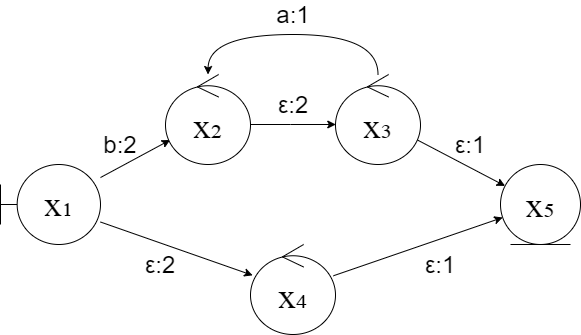
\includegraphics[width=12cm]{../figures/RDLT Weak.png}
    \caption{An RDLT of Weak Soundness (Image Source: \cite{Ramirez2024})}
    \label{RDLTWeak}
\end{figure}

% ---------------------------
% Easy Soundness Notion of RDLTs
\section{Easy Soundness Notion of RDLTs}

\begin{defn}\textbf{Self-Controlling Arc}
    \label{SelfCA}
    A self-controlling arc is a profile of an RDLT $ R $ where a MIX-JOIN or AND-JOIN at vertex $ x $ can never be resolved. 
\end{defn}

Figure \ref{SelfControllingArc}, shown below, is an example of a self-controlling arc as defined in Definition \ref{SelfCA}. In this case, vertex $ b $ is the vertex that can never resolved due to one of the components of the AND-JOIN that violates the unconstrainedness criterion of the activity extraction algorithm.

\begin{figure}[H]
    \centering
    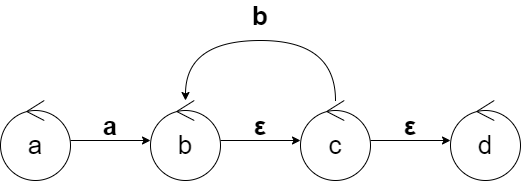
\includegraphics[width=12cm]{../figures/Self-Controlling Loop.png}
    \caption{An RDLT of Easy Soundness Image Source: \cite{Ramirez2024}}
    \label{SelfControllingArc}
\end{figure}

\begin{defn}\textbf{Easy Soundness of RDLTs}
    \label{EasyRDLTDef}
    An RDLT $ R $ is of easy soundness if and only if the following requirement is satisfied by an existing activity profile $ S = \{S(1), S(2), ..., S(k)\}, 1 \leq k \leq diam(R), diam(R) $ is the diameter of $ R $, of a set of source vertices $ I $ $ \subset $ $ V $ and a final output vertex $ f $ $ \in $ $ V, $ where $ \forall $ $ x $ $ \in $ $ I $ and $ y $ $ \in $ $ V $, $ (x,y) $ $ \in $ $ S(1), $ and $ (u,f) $ $ \in $ $ S(k) $, $ u $ $ \in $ $ V $:
    \begin{enumerate}
        \item \textbf{Option to complete.} There exists an activity profile $ S = \{S(1), S(2), ..., S(k)\}, 1 \leq k \leq diam(R) $, of a set of source vertices $ I $ $ \subset $ $ V $ and a final output vertex $ f $ $ \in $ $ V $ where there exists a path $ P $ composed of $ P = x_1, x_2 \cdots x_n $ with $ i = 1, 2 \cdots n - 2 $ where $ (x_i, x_{i+1}) $ $ \in $ $ S(i), (x_{i+1}, x_{i+2}) $ $ \in $ $ S(j), i < j, x_i = s $ and $ x_n = f $.
    \end{enumerate}
\end{defn}

As described in this definition, the only requirement for any given RDLT to be easy sound its sink to be reachable from the source. It does not require proper termination that all reached vertices must have a path that eventually leads to the sink, unlike weak soundness \ref{WeakRDLTDef}. Figure \ref{RDLTEasynotLazy} shows an easy sound RDLT. A deadlock exist due to $x_2$ since there is no path from this vertex that will reach the sink $x_6$. However, there still exist a path from $x_1$ to the sink $x_6$ through the arcs $(x_1,x_5)$, $(x_5,x_6)$, fulfilling the requiremnts for an easy sound RDLT.

\begin{figure}[H]
    \centering
    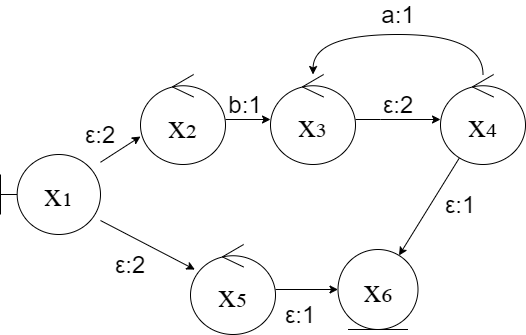
\includegraphics[width=12cm]{../figures/RDLT Easy.png}
    \caption{An RDLT of Easy Soundness Image Source: \cite{Ramirez2024}}
    \label{RDLTEasy}
\end{figure}

\begin{rem}
    Within the context of WF-Nets, the difference between lazy and easy soundness is the number of completed cases where each case instance is represented by a token. Specifically, lazy soundness requires that there should be only one token that reaches the sink place while easy soundness allows multiple tokens in the sink place.
    
    Currently, the activity extraction algorithm for RDLTs, as described in \cite{Malinao2017}, is within the sequential context and therefore only represents one continuous case. With this, it is concluded that, sequentially, the definition of lazy and easy soundness are the same. However, lazy and easy soundness of RDLTs can be differentiated with the use of parallel activity extraction as multiple parallel cases can be visualized through this \cite{Doñoz2024}. This difference is shown in Figure \ref{RDLTEasynotLazy} with the sequential and parallel activity profiles. For the parallel activity, a traversal tree is utilized to visualize the various activities that are happening simultaneously. This visualization aims to structurally show and identify the parallel and non-parallel activities through observing the termination time for each branch as proposed in \cite{Doñoz2024}.

    \begin{figure}[H]
        \centering
        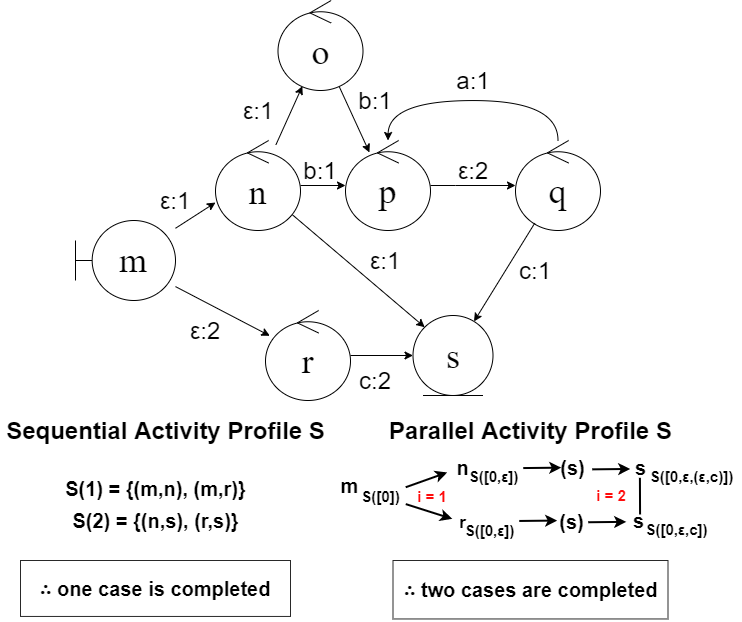
\includegraphics[width=16cm]{../figures/RDLT Parallelized Easy not Lazy w Exp.png}
        \caption{An Parallelized RDLT of Easy but not Lazy Soundness (Image Source: \cite{Ramirez2024})}
        \label{RDLTEasynotLazy}
    \end{figure}
\end{rem}
% ---------------------------
% Behavioral Profiles of Weak and Easy Soundness of RDLTs
\section{Behavioral Profiles of Weak and Easy Sound RDLTs}

This section introduces theorems that define the behavioral profiles of both weak-sound and easy-sound RDLTs.

\begin{thm}[Implication of Weak Soundness from Classical Soundness of an RDLT $ R $] 
    \label{CtWRDLT}
    If an RDLT $ R $ is of classical sound, then it is of weak sound.
\end{thm}

\begin{proof}
    Let $ R $ be a classical sound RDLT.

    Assume that $ R $ is not of weak sound. With this, then the following claim must hold:

    \begin{enumerate}
        \item There exists an activity profile $ S = \{S(1), S(2), ..., S(k)\}, (q,o) $ $ \in $ $ S(k), q $ $ \in $ $ V, k $ $ \in $ $ \mathbb{N}, $ in $ R, $ where $ \exists (p, u) $ $ \in $ $ S(i), 1 \leq i < k, $ such that $ \nexists(u,y) $ $ \in $ $ \bigcup_{j=i+1}^{k} S(j) $. This means that $ S $ does not properly terminate through $ (p,u) $ $ \in $ $ S(i) $, i.e. the child $ y $ $ \in $ $ V $ of $ u $ is a pending task of an unfinished process in $ S $.
    \end{enumerate}
    % For this claim, $ (p,u) $ can either have the following cases:

    % \begin{enumerate}
    %     \item $ (p,u) $ leads to an AND-join merging at $ y $ $ \in $ $ V $, where $ \exists(v,y) $ $ \in $ $ E $, where $ C(u,y) $ 
    %     $ \in $ $ \Sigma, C(u,y) $ $ \neq $ $ C(v,y) $, and an unchecked $ C(v,y) $ results in an unresolved AND-join at y. Through this, both $ (u,y) $ and $ (v,y) $ were never traversed by the algorithm such that there exists a reachability configuration $ S(j) $ where $ (u,y), (v,y) $ $ \in $ $ S(j) $ and $ i < j \leq k $.
    %     \item $ (p,u) $ leads to a MIX-join merging at $ y $ $ \in $ $ V $, where $ C(u,y) $ $ = $ $ \varepsilon $, and $ \exists(v,y) $ $ \in $ $ E $, where $ C(v,y) $ $ \in $ $ \Sigma $, such that an unchecked $ C(v,y) $ leads to the conclusion that both arcs are unconstrained, thus including them in $ S $.
    %     \item $ (p,u) $ leads to an OR-join where a path $ P $ leads to an output $ o' $ $ \in $ $ V $, where $ o' $ $ \neq $ $ o $ which is in turn the sink vertex of $ R $. Through this, $ \exists(a,b) $ $ \in $ $ S(n) $ of the activity profile where $ b $ $ \in $ $ V \ \{o\} $.
    % \end{enumerate}

    As proved in Theorem 1 of \cite{MalinaoPJS2023}, an RDLT $ R $ has been proved to terminate properly given that $ R $ is classical-sound. Through this, a classical sound RDLT satisfies the sole requirement of proper termination that an RDLT of weak soundness must have.
\end{proof}
% ---------------------------
% Structural Profiles of Weak and Easy Soundness of RDLTs
% ---------------------------
\begin{thm}[Implication of Easy Soundness from Weak Soundness of an RDLT $ R $] 
    If an RDLT $ R $ is of weak sound, then it is of easy sound.
    \label{WtERDLT}
\end{thm}

\begin{proof}

    Let R be a weak sound RDLT and assume it is not of easy sound. Through this, it is assumed that there is no activity profile that has a path from the source that eventually leads to the sink.
    
    As proven in Theorem \ref{PTWeak}, the given weak-sound self-controlling RDLT was found to have proper termination even without liveness. With this, it was also proven that it had the option to complete as there must exist a path from $ x $ to the sink vertex. Through this, a weak-sound RDLT satisfies the sole requirement of the option to complete that an RDLT of easy soundness must have.
    
\end{proof}

\begin{cor}[Implication of Easy Soundness from Classical Soundness of an RDLT R]
    If an RDLT $ R $ is classical sound, then it is of easy sound.
    \label{CtERDLT}
\end{cor}

\begin{proof}
    Follows from Theorem \ref{CtWRDLT} and \ref{WtERDLT}.
\end{proof}

\section{Structural Profiles of Weak and Easy Sound RDLTs}

This section introduces theorems that define the structural profiles of both weak-sound and easy-sound RDLTs.

\begin{thm}[Proper Termination of an RDLT $ R $ of Weak Soundness] 
    A weak sound RDLT $ R $ properly terminates even without the requirement of liveness.
    \label{PTWeak}
\end{thm}

\begin{proof}

    Let $ R $ be a self-controlling RDLT where deadlocks occur at $(u,y)$. Let $ R $ also be an RDLT of weak soundness.
    
    Due to the existence of deadlocks, $ R $ is considered to be an RDLT that is not live. To prove that a $ R $ still exhibits proper termination, we need to first establish that $ R $ is able to complete through reaching the sink vertex from the source vertex.
    
    In this case, the activity extraction algorithm reaches $ x $ at $S(t)$ through $v$, i.e $(v, x)$ $ \in $  $ S(t)$. If there exists $(u, y) $ $ \in $ $ E $ and $ C(u, y) $ $ \in $ $ \Sigma $, then $ (u,y) $ is constrained. Since $ R $ is of weak soundness, then there must exist a path $ P = x_1, x_2, ... x-{n-2} $ where $ x_1 = x $ and $ x_{n-2} $ $ = $ $ f $, the sink vertex.
    
    As we now have proven the completion of R, we move on to proving its proper termination by assuming that there exists a path $ P $ $ = $ $ x ... f $ and $ P’$ $ = $ $ x ... f $ where $ P $ $ \neq $ $ P’ $ i.e both arrive at the same sink vertex but they overlap with each other. If the components of $ P $ and $ P’ $ are in $ S $, then they form a MIX-join or an AND-join. Moreover, since paths $ P $ and $ P’ $ both complete in $ S $, then both paths complete at the same time which proves proper termination.
    
\end{proof}

As discussed in Chapter 1, \cite{MalinaoPJS2023} verifies the classical soundness of an RDLT if it satisfies the requirements of JOIN-safe $L-$values and $L-$safeness. \cite{Ramirez2024} propsed an algorithm that takes a similar approach that uses the initial requirements and weakening them, allowing the lack of liveness in a given RDLT.
\begin{defn}\textbf{Weakened JOIN-safe $ L $-values}
    \label{WJVals}
    For every split-join pair of arcs $ (u,y) $, $ (v,y) $ $ \in $ $ E $ in an RDLT $ R $, $ (u,y) $ and $ (v,y) $ have weakened JOIN-safe $ L $-values if the following conditions are met:
    \begin{itemize}
        \item For every process with $ C(u,y) $ or $  C(v,y) $ $ = $ $ \varepsilon $
        \begin{enumerate}
            \item CAs are allowed as long as they are safe, i.e there exists a loop-safe non-critical EA for each CA.
            \item Branching out is allowed as resolving its JOIN is not affected by the arc that has a $ C $-value of $ \varepsilon $.
            \item Process interruptions are allowed regardless of the $ C $-values of the interrupting arc.
        \end{enumerate}
        \item For every process with $ C(u,y) $ or $  C(v,y) $ $ = $ $ \Sigma $
        \begin{enumerate}
            \item \textbf{One-split origin for sibling processes merging at an AND- or MIX-JOIN.} There is one common ancestor $ x $ $ \in $ $ V $ for $ u $ and $ v $ such that there are is a pair of sibling processes $ P_u $ $ = $ $ a_1 \ldots a_n $, where $ a_i $ $ = $ $ x $, $ a_{n-1} $ $ = $ $ u $, $ a_n $ $ = $ $ y $, $ a_i $ $ \in $ $ V $, $ 1 < I < n - 2 $, and $ P_v $ $ = $ $ b_1 \ldots b_m $, where $ b_j $ $ = $ $ x $, $ b_{m-1} $ $ = $ $ v $, $ b_m $ $ = $ $ y $, $ b_j $ $ \in $ $ V $, $ 1 < I < m - 2 $.  Since both paths are siblings, then they must have no arcs in common, i.e. they do not intersect except at $ x $ at $ y $; and
            \item \textbf{No unrelated processes.} For every arc $ (a,b) $ $ \in $ $ E $, if $ a $ $ = $ $ x $, where $ x $ is the one common ancestor of $ u $ and $ v $, then there is no path from $ a $ to another vertex $ r $ $ \in $ $ V $ such that for some $ (r,w) $ $ \in $ $ E $, $ w $ $ \neq $ $ y $.
            \item \textbf{No branching out from every related process.} $ 
            \forall q_k $ $ \in $ $ Lit(P_q) $, where $ q $ $ \in $ $ \{u,v\} $, $ 1 \leq k < |Lit(P_q)| $, $ \nexists (q_{k,s}) $ $ \in $ $ E $ where $ s $ $ \in $ $ V \backslash Lit(P_q) $. This is to ensure that the JOIN is resolved.
            \item \textbf{Process interruptions.} With any loss of generality, if the interrupting arc $ (w,v) $ $ \in $ $ E $ has a $ C $-value of $ \varepsilon $, then process interruptions are allowed.
            \item \textbf{Duplicate values.} 
            \begin{itemize}
                \item If $ C(u,y) $, $ C(v,y) $ $ \in $ $ \Sigma $, i.e. an AND-JOIN at $ y $, then there is no process $ P $ $ = $ $ [x_1 x_2 \ldots x_p] $ in $ R $, where $ x_1 $ $ = $ $ x $, $ x_p $ $ = $ $ y $, such that $ C(x_{p-1}, x_p ) $ $ = $ $ C(u,y) $ (or $ C(v,y) $).
                \item Without any loss of generality, if $ C(u,y) $ $ = $ $ \varepsilon $ and $ C(v,y) $ $ \in $ $ \Sigma $, i.e. a MIX-JOIN at $ y $, then any process $ P $ $ = $ $ x_1 x_2 \ldots x_p $ in $ R $, where $ x_1 $ $ = $ $ x $, $ x_p $ $ = $ $ y $, can have $ C(x_{p-1},x_p) $ $ \in $ $ \{ \varepsilon, C(v,y) \} $, i.e. duplicate $ C $-values are allowed but no two of such arcs must have different $ C $-values.
            \end{itemize}
            \item \textbf{Equal $ L $-values of arcs at the AND-JOIN.}
            \item \textbf{No CAs exist within the process.} 
        \end{enumerate}
    \end{itemize}
\end{defn}

In comparison to the requirements of JOIN-safe L-values as described in Definition \ref{JSL}, the requirements for weakened JOIN-safe L-values is more lenient as the name suggests. Specifically, the fourth requirement is weakened such that it now allows process interruptions given that their $ C $-value is equal to $ \varepsilon $. Although it retains the first six requirements from the JOIN-safe L-values definition, it replaces the requirement of the loop-safeness of all related process with the requirement that there are no CAs within the process. Through these changes, this allows deadlocks to occur given that it does not occur within JOINs that has a process with a C-value with $ \Sigma $. 

\begin{defn}\textbf{Weakened JOIN-safe RDLT $ R $}
    \label{WJRDLT}
    An RDLT $ R $ is weakened JOIN-safe if every split-join pair in $ R $ has weakened JOIN-safe $ L $-values.
\end{defn}

\begin{defn}\textbf{Deadlock Point}
    \label{DLP}
    A deadlock point is each vertex $ x $ $ \in $ $ dV $ in an RDLT $ R $ where $ dV $ is a set of vertices in $ R $ and $ dV $ $ \subset $ $ V $, such that $ x $ $ \in $ $ dV $ is unreachable at some time step of the activity extraction algorithm.
\end{defn}

\begin{defn}\textbf{Escape Contraction Path}
    \label{ECPath}
    An escape contraction path is a path $ P = x_1, x_2 \ldots x_n $ in an RDLT $ R $ such that the following holds:
    \begin{enumerate}
        \item $ x_1 $ is a parent of a deadlock point in $ R $, i.e. $ x_1 $ $ = $ $ p $ where $ (p,q) $ $ \in $ $ E $ and $ q $ $ \in $ $ dV $, and
        \item $ P $ is a contraction path from $ x_1 $ to $ x_n $ in $ R $ where $ x_n $ is the sink vertex of $ R $.
    \end{enumerate}
\end{defn}

Definitions \ref{DLP} and \ref{ECPath} both describe the structures that must both exist simultaneously in a weak-sound RDLT as it assures that such an RDLT properly terminates even with the presence of deadlocks. As an example, vertex $ x_2 $ in Figure \ref{RDLTWeak} is the deadlock point of the RDLT as it is unreachable at the first time step of the activity. The escape contraction path in this case is $ P $ $ = $ $ x_1, x_4, x_5 $ where $ x_1 $ is the parent of the deadlock point $ x_2 $ and $ x_5 $ is the sink vertex.

\begin{defn}\textbf{Deadlock-Resolving RDLT $ R $}
    \label{DLResolving}
    An RDLT $ R $ is deadlock-resolving if for every deadlock point $ x \in V $, there exists at least one escape contraction path from a parent of $ x $ to the sink in R.
\end{defn}

\begin{lem}
    An expanded vertex simplification $ R_i $, where $ i $ $ = $ $ 1, 2 $, is deadlock-tolerant if and only if every activity thereof properly terminates.
\end{lem}

\begin{defn}\textbf{Deadlock-Tolerant RDLT $ R $}
    An RDLT $ R $ is deadlock-tolerant if every NCA is loop-safe, every CA is safe, $ R $ is weakened JOIN-safe and deadlock-resolving.
\end{defn}

With these definitions, the structural definition of a weak-sound RDLT is defined in Theorem \ref{SVWeak}.

\begin{thm}\textbf{Structural Verification of the Weak Soundness of an RDLT $ R $}
    \label{SVWeak}
    An RDLT $ R $ is weak-sound if and only if both the level-1 and level-2 expanded vertex simplifications of R, $ R_1 $ and $ R_2 $ respectively, are deadlock-tolerant.
\end{thm}

With Theorem \ref{SVWeak} as the basis, Algorithm \ref{WeakAlg} verifies the weak soundness of a given input RDLT $ R $ through the satisfaction of the requirements of deadlock-tolerance.

\begin{algorithm}[H]
    \caption{Weak RDLT Soundness Verification Algorithm (WRSVA) }
    \label{WeakAlg}
    \begin{algorithmic}
        \State \textbf{Input:} RDLT $ R $ with or without RBS
        \State \textbf{Output:} True, false otherwise
    \end{algorithmic}
    \begin{algorithmic}[1]
        \State Apply Expanded Vertex Simplification Algorithm \cite{MalinaoWCTP2023}
        \If{$ R $ contains an RBS}
            \State $ i $ $ = $ $ 2 $
        \Else
            \State $ i $ $ = $ $ 1 $
        \EndIf
        \For{every vertex simplification $ R_i $}
            \For{every vertex $ v $ $ \in $ $ V $}
                \State Store deadlock point $ y $
            \EndFor
            \For{every deadlock point $ y $ $ \in $ $ V $}
                \State Determine if a non-critical loop-safe escape contraction path exists from $ y $
                \State Determine if the split-join pair containing $ y $ has weakened JOIN-safe L-values
            \EndFor            
        \EndFor
        \If{$ R_1 $ is deadlock-tolerant}
            \If{$ R $ contains an RBS}
                \If{$ R_2 $ deadlock-tolerant}
                    \State \Return true
                \EndIf
            \EndIf
            \State \Return true
        \Else
            \State \Return false
        \EndIf
    \end{algorithmic}
\end{algorithm}

\begin{thm}\textbf{Time Complexity of WRSVA}
    The time complexity of verifying that an RDLT $ R $ is weak-sound is $ O(c|E|^4) $.
    \label{TCWRSVA}
\end{thm}
\begin{proof}
    The algorithm is divided into three main processes: (1) expanded vertex simplification \cite{MalinaoWCTP2023}, (2) determining the deadlock-points, and (3) verifying deadlock tolerance. For the first process, it has a time complexity of $ O(|V|^2)$ which corresponds to the maximum number of arcs $ R $ can have. Because the algorithm visits every arc of the diagram to replicate them or create abstract versions for the outputs $ R_1 $ and $ R_2 $ (if an RBS exists), the worst-case scenario for this algorithm is when the RDLT has the maximum amount of arcs, hence $ O(|V|^2) $. 
    
    For the second process, it has a time complexity of $ O(|V|+|E|)$, where it corresponds to the sum of the number of vertices $ V $ and arcs $ E $ in $ R $. This process uses the depth-first or breadth-first search algorithm to solve the problem, hence $ O(|V|+|E|) $.

    The third process of verifying deadlock tolerance can be divided into its four requirements which has their own processes: (1) verifying loop-safeness, which takes $ O(c|E|^4) $ time \cite{MalinaoPJS2023}, (2) verifying existence of safe critical arcs, which takes $ O(|E|^2) $ time \cite{MalinaoPJS2023}, (3) verifying weakened JOIN-safeness, and (4) verifying deadlock resolution.
    
    The verification of weakened JOIN-safeness can be further divided into its component processes and determining each of their time complexities. Specifically for every AND- and MIX-JOIN, it concerns the processes of (1) determining the one split origin, (2) determining if there are no unrelated process, (3) determining if there are no branches, (4) determining if there are no processes interruptions with a C-value of $ Sigma $, (5) determining duplicate conditions at the merge point, (6) determining the equality of the L-values, and (7) determining the non-existence of critical arcs. The first three processes take $ O(|V||E|^2) $ time \cite{MalinaoPJS2023}. The fourth process takes $ O(|V||E|) $ time, similar to its stricter counterpart in \cite{MalinaoPJS2023} where it avoids all process interruptions no matter the $ C $-attribute. The fifth and sixth processes takes $ O(|V||E|log|E|) $ and $ O(|V||E|) $ time respectively \cite{MalinaoPJS2023}. The last process to determine the number takes $ O(c|E|) $ where $ c $ is the number of cycles as it is the highest time complexity of the required steps to find so, specifically Problem 1 to 3 in Lemma 1 of \cite{Malinao2017}. Because the dominating processes in terms of time complexity are the first three processes, the time complexity of verifying weakened JOIN-safeness is $ O(|V||E|^2) $.

    Lastly, verifying if the RDLT $ R $ is deadlock-resolving requires $ O(p(|V| + |E|)) $ where $ p $ signifies the number of deadlock points since deadlock-resolving is essentially the process of graph contraction, which takes $ O(|V| + |E|) $ \cite{MalinaoPJS2023}, for every deadlock point in $ R $.
    
    With the time complexities of the sub-processes of deadlock tolerance, verifying loop-safeness has the greatest complexity out of the processes, making the time complexity of determining deadlock tolerance is $ O(c|E|^4) $.

    Since the time complexity of the determining deadlock tolerance is greater out of the processes as well, the weak soundness of $ R $ can be determined in $ O(c|E|^4) $ time.
\end{proof}

\begin{thm}\textbf{Space Complexity of WRSVA}
    The space complexity of verifying that an RDLT $ R $ is weak-sound is $ O(|E|^2) $.
    \label{SCWRSVA}
\end{thm}
\begin{proof}
    As mentioned earlier, the algorithm is divided into three main processes. For the first process of EVS, it has a space complexity of $ O(|V|^2)$ which corresponds to the maximum number of arcs $ R $ can have. Because the algorithm stores every arc of the diagram to replicate them or create abstract versions for the outputs $ R_1 $ and $ R_2 $ (if an RBS exists), the worst-case scenario for this algorithm is when the RDLT has the maximum amount of arcs, hence $ O(|V|^2) $. 
    
    For the second process, it has a space complexity of $ O(|V|+|E|)$ similar to its time complexity. It stores the vertices and arcs traversed to create the contraction path as it uses the depth-first or breadth-first search algorithm to solve the problem, hence $ O(|V|+|E|) $.

    The third process of verifying deadlock tolerance can be divided into its four requirements which has their own processes: (1) verifying loop-safeness, which takes $ O(c|E|) $ space \cite{MalinaoPJS2023}, (2) verifying existence of safe critical arcs, which takes $ O(|v|+|E|) $ space \cite{MalinaoPJS2023}, (3) verifying weakened JOIN-safeness, and (4) verifying deadlock resolution.
    
    The verification of weakened JOIN-safeness can be further divided into its component processes and determining each of their space complexities. Specifically for every AND- and MIX-JOIN, it concerns the processes of (1) determining the one split origin, (2) determining if there are no unrelated process, (3) determining if there are no branches, (4) determining if there are no processes interruptions with a C-value of $ Sigma $, (5) determining duplicate conditions at the merge point, (6) determining the equality of the L-values, and (7) determining the non-existence of critical arcs. The first five processes as well as the last process use $ O(|E|^2) $ space \cite{MalinaoPJS2023}. However, the sixth process uses $ O(|V||E|) $ space. Because the sixth process needs the least amount of space and is the sole process with a different complexity, the space complexity of verifying weakened JOIN-safeness is $ O(|E|^2) $.

    Lastly, verifying if the RDLT $ R $ is deadlock-resolving requires $ O(p(|V| + |E|)) $ space similar to its time needed as this process is similar to the graph contraction for every deadlock point in $ R $.
    
    With the space complexities of the sub-processes of deadlock tolerance, verifying loop-safeness has the greatest complexity out of the processes, making the time complexity of determining deadlock tolerance is $ O(|E|^2) $.

    Since the space complexity of the determining deadlock tolerance is greater out of the processes as well, the weak soundness of $ R $ can be determined with $ O(|E|^2) $ space.
\end{proof}

Shown below is Theorem \ref{SVEasy} that describes the structural requirements required to determine the easy soundness of an RDLT.

\begin{thm}\textbf{Structural Verification of the Easy Soundness of an RDLT $ R $}
    \label{SVEasy}
    An RDLT $ R $ is easy-sound if and only if the following elements exist: 
    \begin{itemize}
        \item A contraction path $ P_1 $ in the level-1 vertex simplification $ R_1 $ of $ R $ from the initial vertex $ x_i $ to the final vertex $ x_f $, wherein $ P_1 $ $ = $ $ x_1, \ldots, x_f $
        \item A contraction path $ P_2 $ in the level-2 vertex simplification $ R_2 $ of $ R $ from the initial vertex $ z $ to the final vertex $ p $ of the RBS, wherein $ P_2 $ $ = $ $ z, \ldots, p $
        \item An in-bridge $ (x,y) $ formed by a component in $ P_1 $ such that there exists a component $ (y,z) $ in $ P_2 $
        \item An out-bridge $ (q,p) $ formed by a component in $ P_2 $ such that there exists a component $ (p,r) $ in $ P_1 $
    \end{itemize}
\end{thm}

With Theorem \ref{SVEasy} as the basis, Algorithm \ref{EasyAlg} verifies the easy soundness of a given input RDLT $ R $ through the satisfaction of a contraction path existing from the source to the sink vertex.

\begin{algorithm}[H]
    \caption{Easy RDLT Soundness Verification Algorithm (ERSVA) }
    \label{EasyAlg}
    \begin{algorithmic}
        \State \textbf{Input:} RDLT $ R $ with or without RBS
        \State \textbf{Output:} True, false otherwise
    \end{algorithmic}
    \begin{algorithmic}[1]
        \State Apply Vertex Simplification Algorithm \cite{Malinao2017}
        \If{$ R $ contains an RBS}
            \State $ i $ $ = $ $ 2 $
        \Else
            \State $ i $ $ = $ $ 1 $
        \EndIf
        \For{every vertex simplification $ R_i $}
            \State Apply Graph Contraction Strategy \cite{Malinao2017}
        \EndFor
        \If{$ R_1 $ has a contraction path from the source $ x_1 $ to the sink $ x_n $}
            \If{$ R $ contains an RBS}
                \If{$ R_2 $ has a contraction path from the source $ z $ to the sink $ p $}
                    \State \Return true
                \EndIf
            \EndIf
            \State \Return true
        \Else
            \State \Return false
        \EndIf
    \end{algorithmic}
\end{algorithm}

To illustrate this verification of easy soundness, Figure \ref{VSEasy} depicts the step-by-step application of ERSVA to the easy sound RDLT shown in Figure \ref{RDLTEasy}. Since such an RDLT does not have an RBS, then it represents the level-1 vertex simplification and does not have a level-2 vertex simplification. Although this contraction does not result in one singular vertex representing all the vertices in the original figure, there exists a contraction path from the initial vertex $ x_1 $ to the final vertex $ x_6 $. This proves that the option to complete requirement is satisfied by the RDLT, thus verifying its easy soundness.

    \begin{figure}[H]
        \centering
        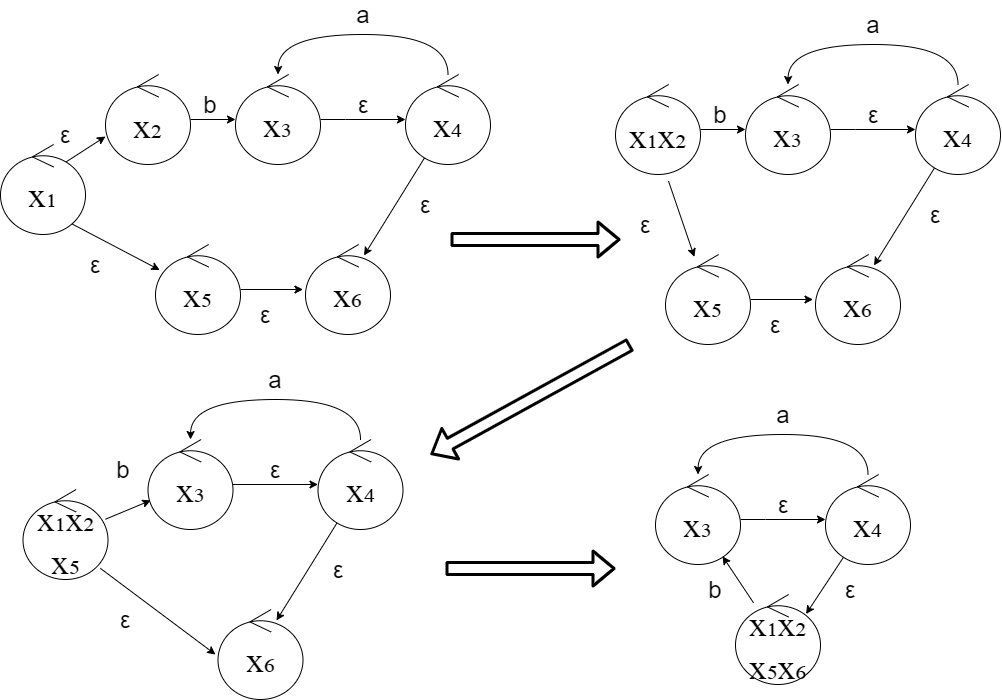
\includegraphics[width=15cm]{../figures/SV Easy Sound RDLT.png}
        \caption{An Parallelized RDLT of Easy but not Lazy Soundness}
        \label{VSEasy}
    \end{figure}

\begin{thm}\textbf{Time Complexity of ERSVA}
    The time complexity of verifying that an RDLT $ R $ is easy-sound is $ O(|V|^2) $.
    \label{TCERSVA}
\end{thm}
\begin{proof}
    The algorithm is divided into two main processes: (1) vertex simplification \cite{Malinao2017} and (2) graph contraction \cite{Malinao2017, MalinaoPJS2023}. For the first process, it has a time complexity of $ O(|V|^2)$ which corresponds to the maximum number of arcs $ R $ can have. Because the algorithm visits every arc of the diagram to replicate them or create abstract versions for the outputs $ R_1 $ and $ R_2 $ (if an RBS exists), the worst-case scenario for this algorithm is when the RDLT has the maximum amount of arcs, hence $ O(|V|^2) $. 
    
    For the second process, it has a time complexity of $ O(|V|+|E|)$, where it corresponds to the sum of the number of vertices $ V $ and arcs $ E $ in $ R $, because the process essentially determines if there exists a path from the source vertex to every vertex. Although this process is only done to make sure that there is a path from the source to the sink vertex, this complexity still applies as a worst-case scenario when there are no deadlocks within $ R $, i.e. $ R $ is live. As proved in \cite{MalinaoPJS2023}, this process uses the depth-first or breadth-first search algorithm to solve the problem, hence $ O(|V|+|E|) $.

    Since the time complexity of the vertex simplification is greater out of the two processes, the easy soundness of $ R $ can be determined in $ O(|V|^2) $ time.
\end{proof}

\begin{thm}\textbf{Space Complexity of ERSVA}
    \label{SCERSVA}
    The space complexity of verifying that an RDLT $ R $ is easy-sound is $ O(|V|^2) $.
\end{thm}
\begin{proof}
    Similar to the time complexity, the algorithm is divided into the vertex simplification and graph contraction. 
    
    For the first process, it has a space complexity of $ O(|V|^2)$ as the process stores every arc within $ R $ to generate $ R_1 $ and $ R_2 $ if $ R $ has an RBS. The worst-case scenario is $ R $ having the maximum amount of arcs given a number of vertices $ V $,  hence $ O(|V|^2) $. 

    For the second process, it has a space complexity of $ O(|V| + |E|) $ \cite{MalinaoPJS2023} as the process stores the vertices and arcs to simulate the possible contraction path of both the vertex simplifications. 

    Since the space complexity of the vertex simplification is greater out of the two processes, the easy soundness of $ R $ can be determined using $ O(|V|^2) $ space.
\end{proof}
\newpage
\section*{On the Matrix Representation of the Verification of Soundness}
\subsection*{}